\documentclass[twoside]{homework}

\usepackage{dsfont} 
\usepackage{subfigure} 
\usepackage{graphicx}
\usepackage{listings}
\usepackage{xcolor}
\lstset{
    rulesepcolor= \color{gray}, %代码块边框颜色
    breaklines=true,  %代码过长则换行
    numbers=left, %行号在左侧显示
    numberstyle= \small,%行号字体
    %keywordstyle= \color{red},%关键字颜色
    commentstyle=\color{gray}, %注释颜色
    frame=shadowbox%用方框框住代码块
}

\studname{Chenye Yang}
\uni{cy2540}
\studmail{cy2540@columbia.edu}
\coursename{ELEN E6880: RMT with Applications}
\hwNo{0}

\begin{document}
\maketitle

\section*{P1}
\subsection*{(a)}
\textbf{Code:}
\begin{lstlisting}[language={Matlab}]
clear;clc;
K = 10000;
N = 20;

mu = 0;         % mean value
var = 1/N;      % variance
sd = sqrt(var); % standard deviation 
A = cell(1, K);

% Creat an ensemble of K realizations of N x N Gaussian symmetric matrices
for i = 1:1:K                       % index to an ensemble of K realizations
    for j = 1:1:N                   % index to row of one matrix
        for k = j:1:N               % index to column of one matrix
            A{i}(j,k) = normrnd(mu,sd);
            A{i}(k,j) = A{i}(j,k);  % make the matrix symmetric
        end
    end
end

e = zeros(N,K);
for i = 1:1:K
    e (:, i) = eig(A{i});
end

% Plot a histogram with Normalization set to 'pdf' to produce an estimation of the probability density function.
histogram(e, 'Normalization','pdf') 
ylabel('Frequency / Width');
xlabel('Eigenvalues');
title('Averaged Histograms, K=10000, N=20');
saveas(gcf,'/Users/yangchenye/Downloads/HW0_1_a_10000_20.png')
\end{lstlisting}
\textbf{Result:}
\begin{figure*}[!h]
\centering
\subfigure[K = 10000, N = 5]{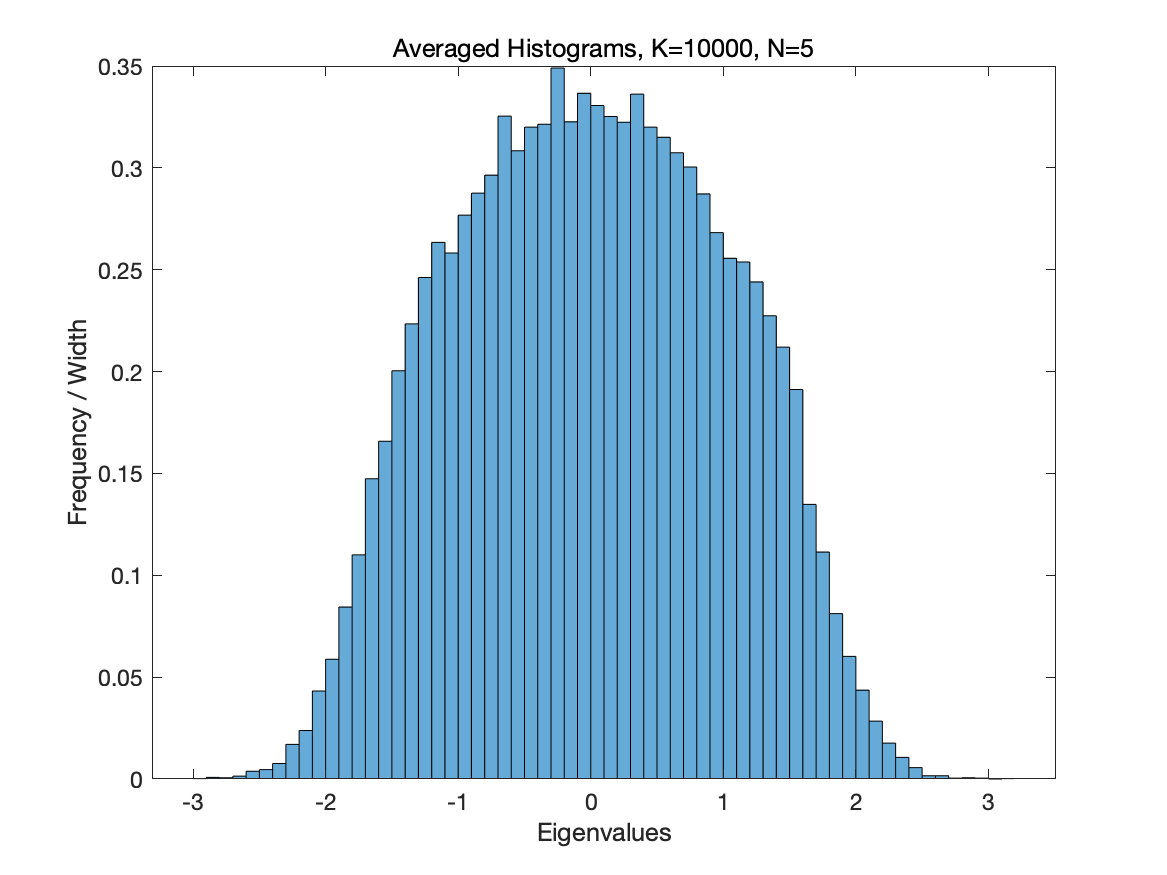
\includegraphics[width=0.49\textwidth]{HW0_1_a_10000_5.png}}
\subfigure[K = 10000, N = 20]{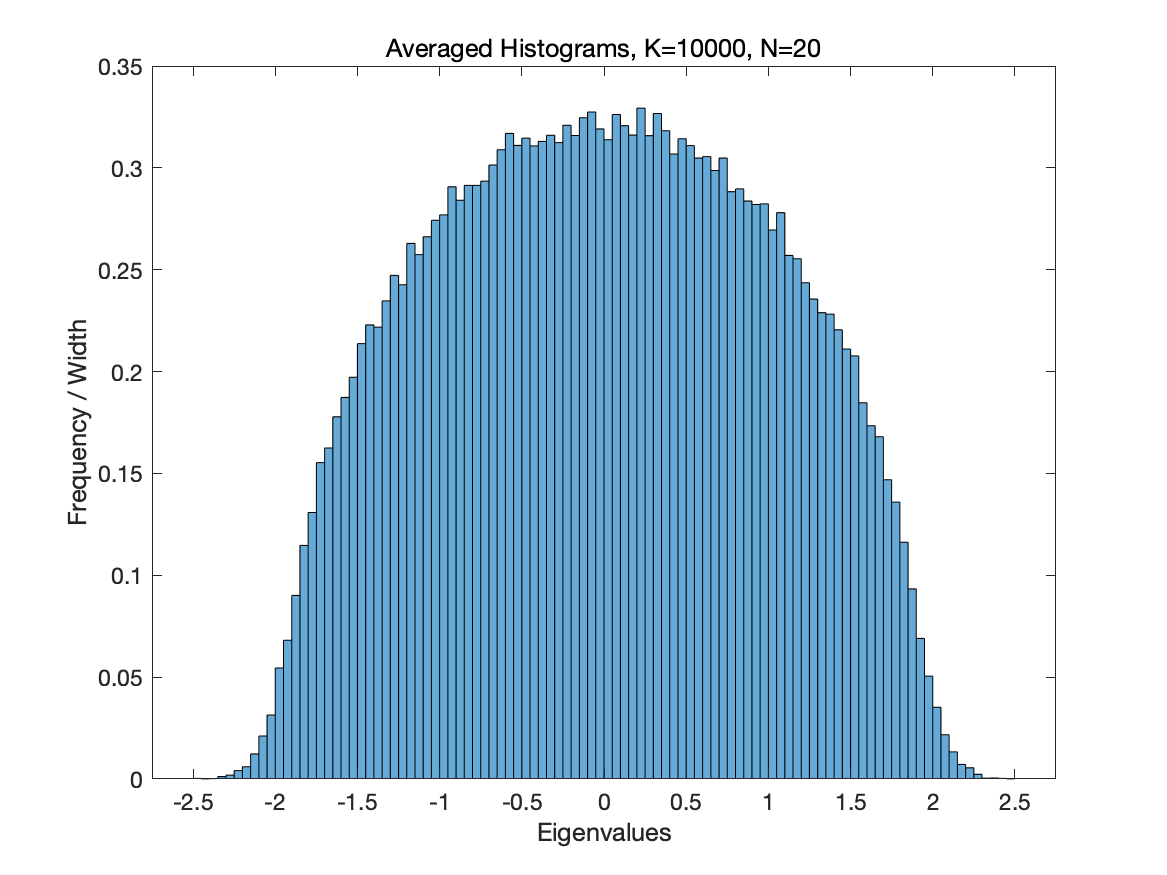
\includegraphics[width=0.49\textwidth]{HW0_1_a_10000_20.png}}
\caption{Averaged histograms of the eigenvalues of A}
%\label{fig1}
\end{figure*}

\subsection*{(b)}
\textbf{Code:}
\begin{lstlisting}[language={Matlab}]
clear;clc;
K = 1;
N = 4000;

mu = 0;         % mean value
var = 1/N;      % variance
sd = sqrt(var); % standard deviation 
A = cell(1, K);

% Creat an ensemble of K realizations of N x N Gaussian symmetric matrices
for i = 1:1:K                       % index to an ensemble of K realizations
    for j = 1:1:N                   % index to row of one matrix
        for k = j:1:N               % index to column of one matrix
            A{i}(j,k) = normrnd(mu,sd);
            A{i}(k,j) = A{i}(j,k);  % make the matrix symmetric
        end
    end
end

e = zeros(N,K);
for i = 1:1:K
    e (:, i) = eig(A{i});
end

% Plot a histogram with Normalization set to 'pdf' to produce an estimation of the probability density function.
histogram(e,'Normalization','pdf')
ylabel('Frequency / Width');
xlabel('Eigenvalues');
title('Averaged Histograms, K=1, N=4000');
saveas(gcf,'/Users/yangchenye/Downloads/HW0_1_b_1_4000.png')
\end{lstlisting}
\textbf{Result:}
\begin{figure*}[ht]
\centering
\subfigure[K = 1, N = 10]{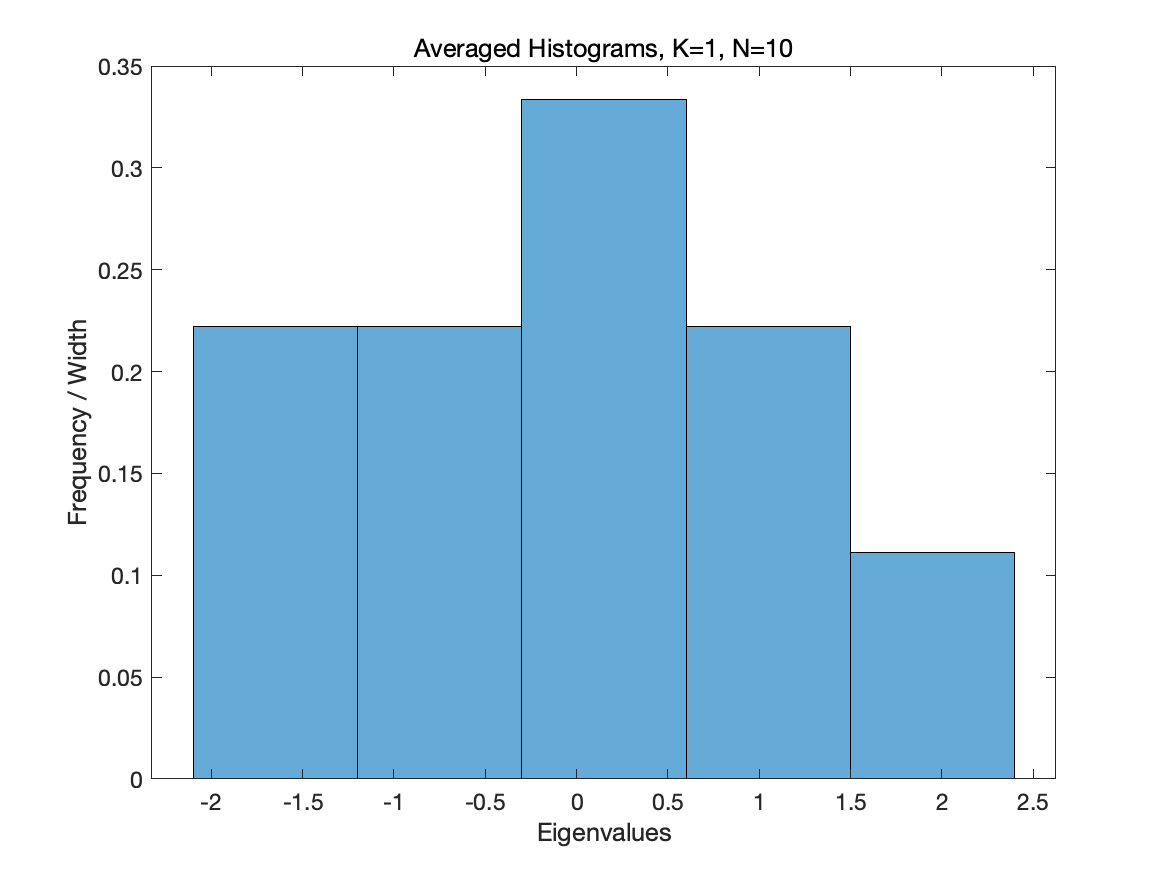
\includegraphics[width=0.49\textwidth]{HW0_1_b_1_10.png}}
\subfigure[K = 1, N = 100]{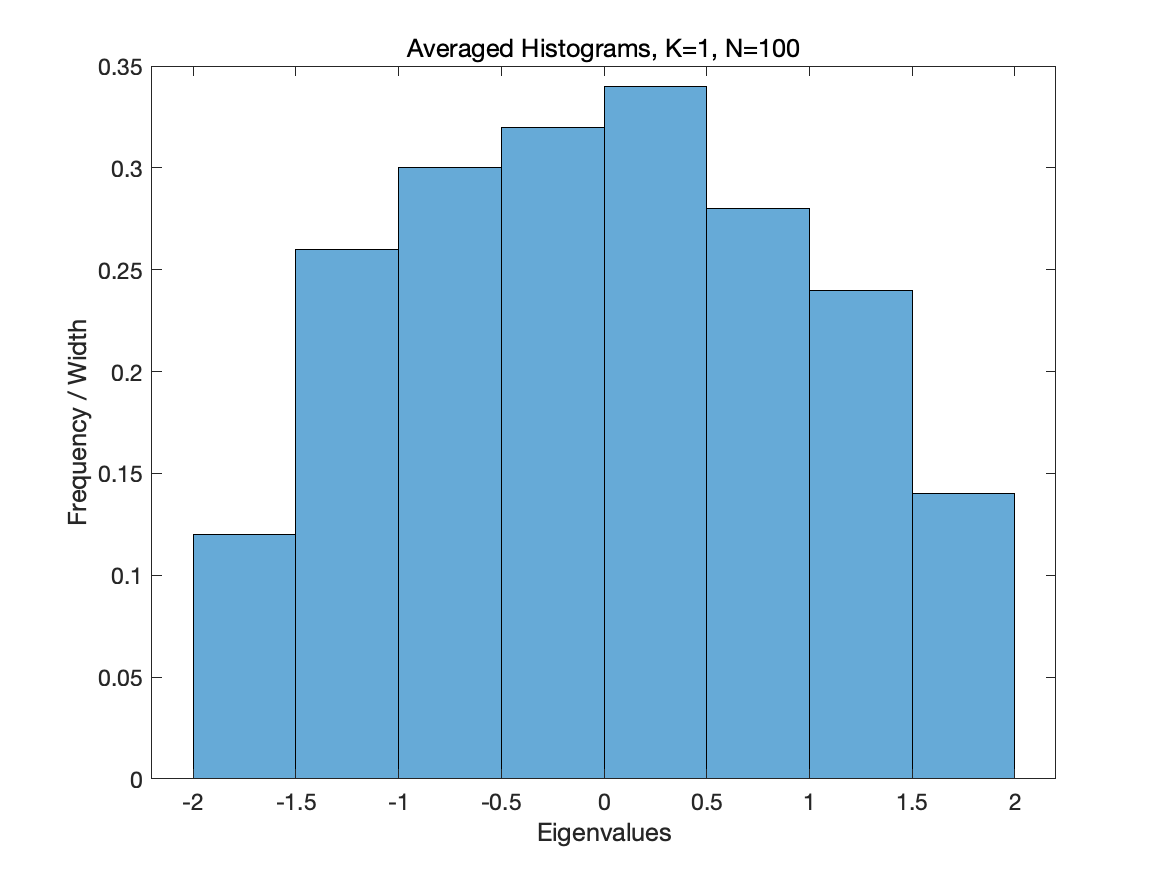
\includegraphics[width=0.49\textwidth]{HW0_1_b_1_100.png}}
\subfigure[K = 1, N = 1000]{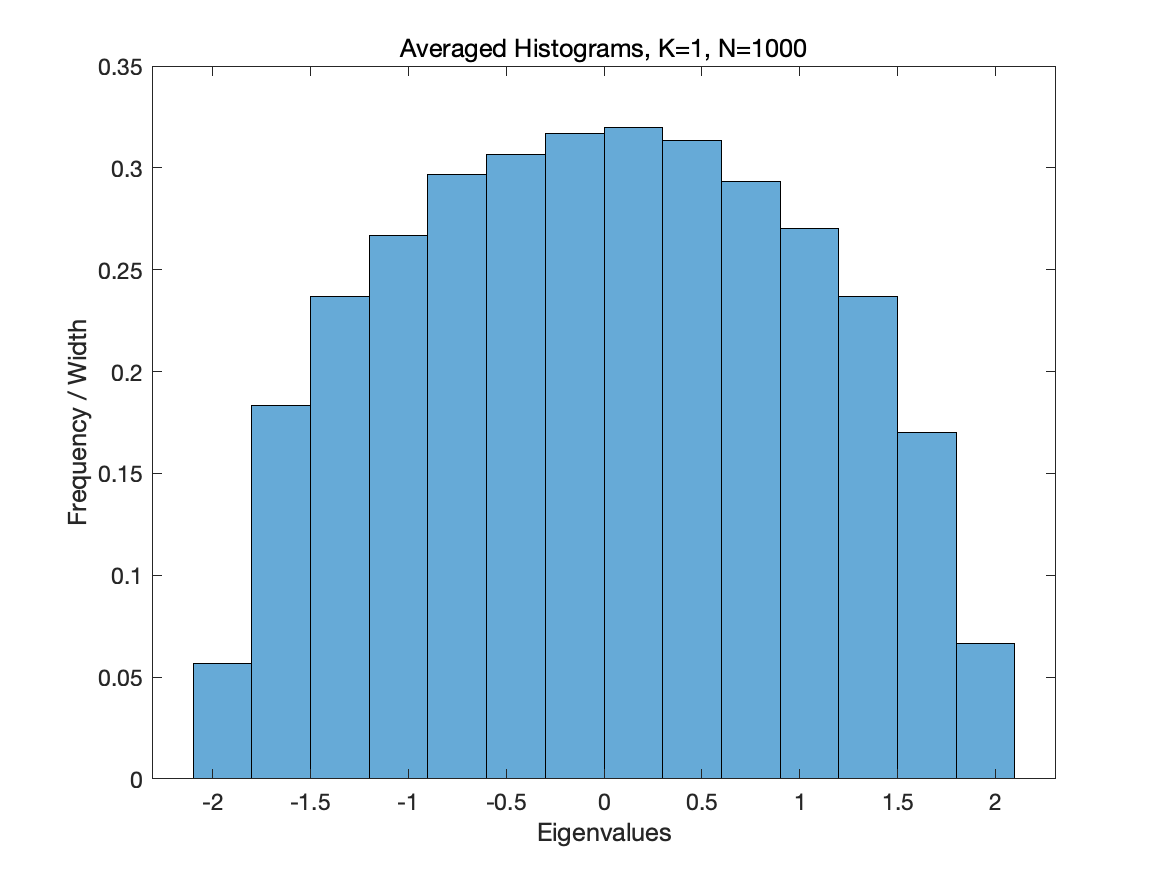
\includegraphics[width=0.49\textwidth]{HW0_1_b_1_1000.png}}
\subfigure[K = 1, N = 4000]{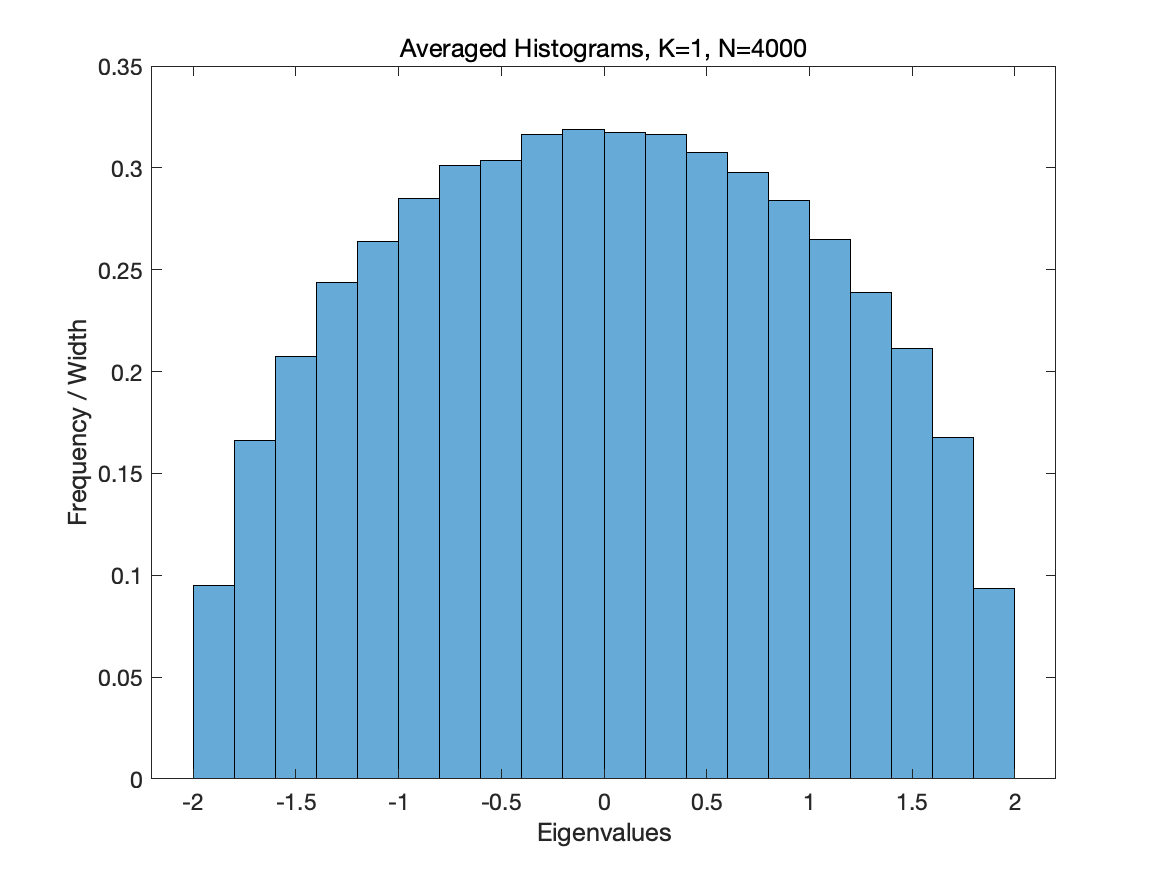
\includegraphics[width=0.49\textwidth]{HW0_1_b_1_4000.png}}
\caption{Averaged histograms of the eigenvalues of A}
%\label{fig1}
\end{figure*}

\subsection*{(c)}
\textbf{Code:}
\begin{lstlisting}[language={Matlab}]
function [p] = Wigner(lamda)
% the analytical curve (Wigner's semi-circle law of the limiting distribution)
for l = 1:length(lamda)
    p(l) = (1/(2*pi))*sqrt(4-lamda(l)^2)*(abs(lamda(l))<2);
end
\end{lstlisting}
\begin{lstlisting}[language={Matlab}]
% a
clear;clc;
KK1 = [10000];
NN1 = [5, 20];

for kindex = 1:length(KK1)
    for nindex = 1:length(NN1)
        
        K = KK1(kindex);
        N = NN1(nindex);

        mu = 0;         % mean value
        var = 1/N;      % variance
        sd = sqrt(var); % standard deviation 
        A = cell(1, K);

        % Creat an ensemble of K realizations of N x N Gaussian symmetric matrices
        for i = 1:1:K                       % index to an ensemble of K realizations
            for j = 1:1:N                   % index to row of one matrix
                for k = j:1:N               % index to column of one matrix
                    A{i}(j,k) = normrnd(mu,sd);
                    A{i}(k,j) = A{i}(j,k);  % make the matrix symmetric
                end
            end
        end

        e = zeros(N,K);
        for i = 1:1:K
            e (:, i) = eig(A{i});
        end
        % Plot a histogram with Normalization set to 'pdf' to produce an estimation of the probability density function.
        histogram(e, 'Normalization','pdf')
        ylabel('p(\lambda)');
        xlabel('\lambda');
        title(['Averaged Histograms, K=',num2str(K),', N=',num2str(N)]);
        hold on
        plot([-3:0.1:3], Wigner([-3:0.1:3]), '-r', 'linewidth', 2);
        legend('histograms','analytical curve');
        saveas(gcf,['/Users/yangchenye/Downloads/HW0_1_c_',num2str(K),'_',num2str(N),'.png'])
        close;
    end
end


% b
clear;clc;
KK2 = [1];
NN2 = [10, 100, 1000, 4000];

for kindex = 1:length(KK2)
    for nindex = 1:length(NN2)
        
        K = KK2(kindex);
        N = NN2(nindex);

        mu = 0;         % mean value
        var = 1/N;      % variance
        sd = sqrt(var); % standard deviation 
        A = cell(1, K);

        % Creat an ensemble of K realizations of N x N Gaussian symmetric matrices
        for i = 1:1:K                       % index to an ensemble of K realizations
            for j = 1:1:N                   % index to row of one matrix
                for k = j:1:N               % index to column of one matrix
                    A{i}(j,k) = normrnd(mu,sd);
                    A{i}(k,j) = A{i}(j,k);  % make the matrix symmetric
                end
            end
        end

        e = zeros(N,K);
        for i = 1:1:K
            e (:, i) = eig(A{i});
        end
        % Plot a histogram with Normalization set to 'pdf' to produce an estimation of the probability density function.
        histogram(e, 'Normalization','pdf') 
        ylabel('p(\lambda)');
        xlabel('\lambda');
        title(['Averaged Histograms, K=',num2str(K),', N=',num2str(N)]);
        hold on
        plot([-3:0.1:3], Wigner([-3:0.1:3]), '-r', 'linewidth', 2);
        legend('histograms','analytical curve');
        saveas(gcf,['/Users/yangchenye/Downloads/HW0_1_c_',num2str(K),'_',num2str(N),'.png'])
        close;
    end
end
\end{lstlisting}
\textbf{Result:}
\begin{figure*}[!h]
\centering
\subfigure[K = 10000, N = 5]{\label{subfig:c_a_1}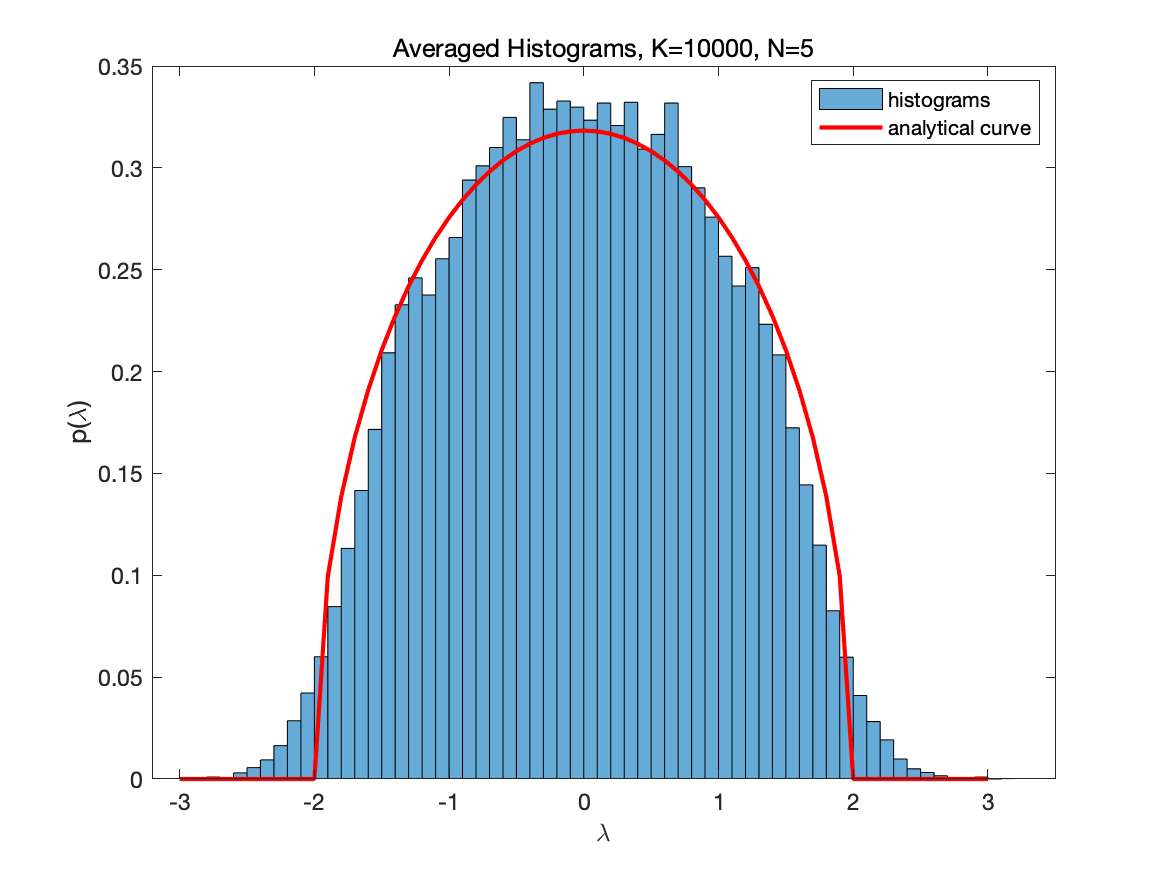
\includegraphics[width=0.49\textwidth]{HW0_1_c_10000_5.png}}
\subfigure[K = 10000, N = 20]{\label{subfig:c_a_2}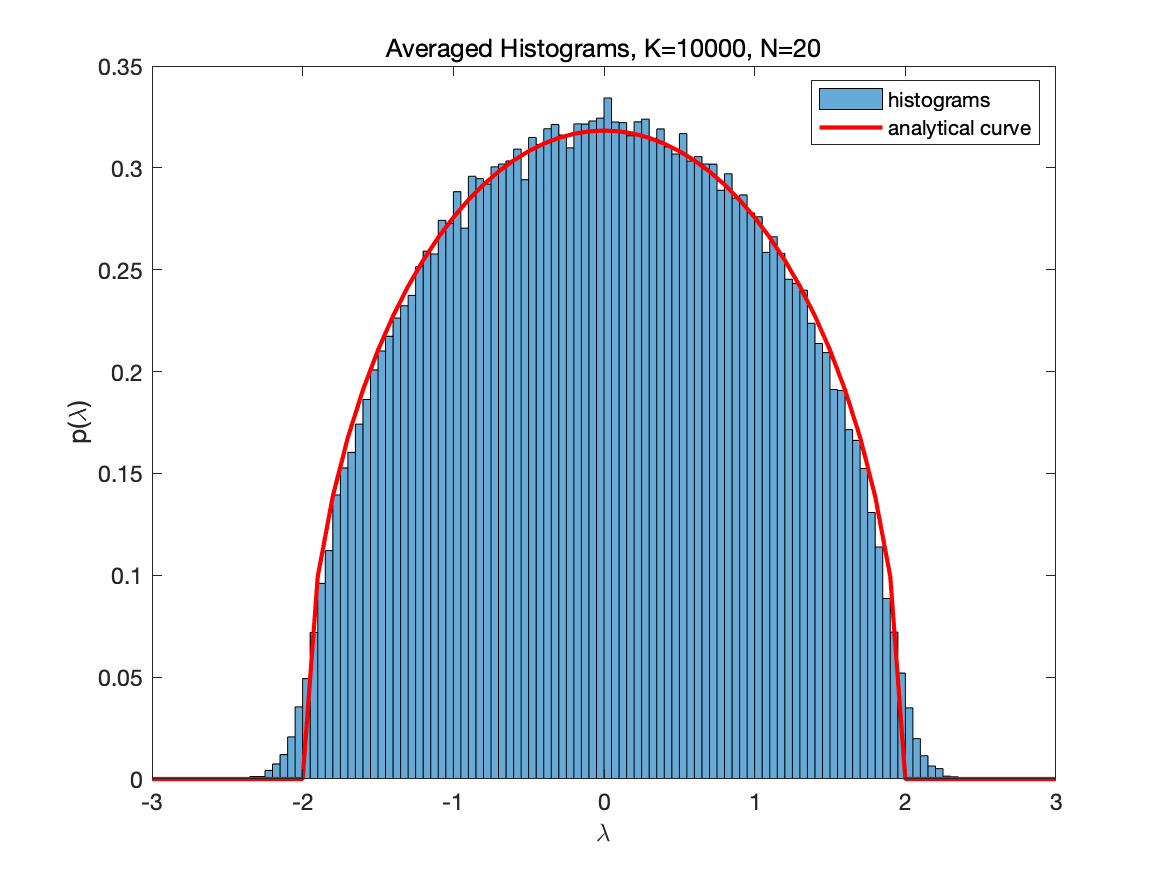
\includegraphics[width=0.49\textwidth]{HW0_1_c_10000_20.png}}
\caption{Averaged histograms and analytical curve, convergence (a)}
\label{fig:c_a}
\end{figure*}
\begin{figure*}[!h]
\centering
\subfigure[K = 1, N = 10]{\label{subfig:c_b_1}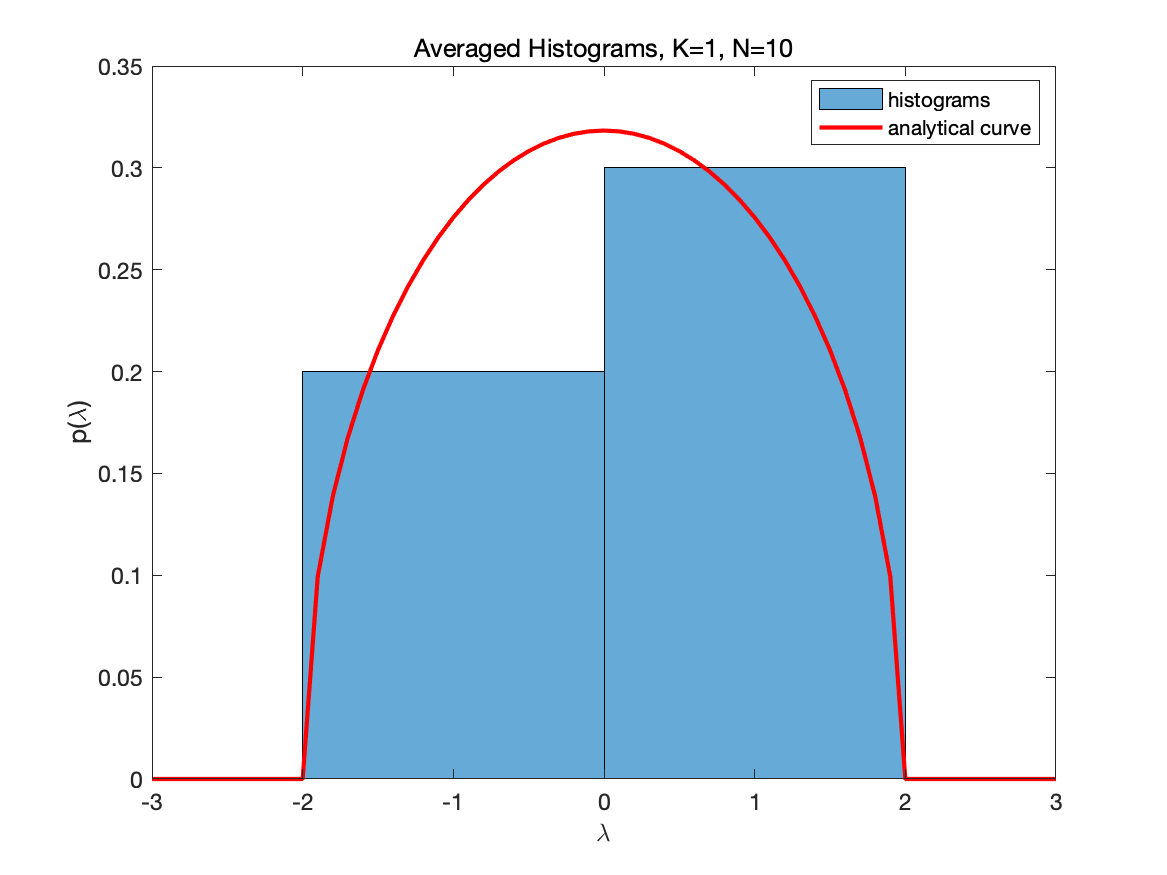
\includegraphics[width=0.49\textwidth]{HW0_1_c_1_10.png}}
\subfigure[K = 1, N = 100]{\label{subfig:c_b_2}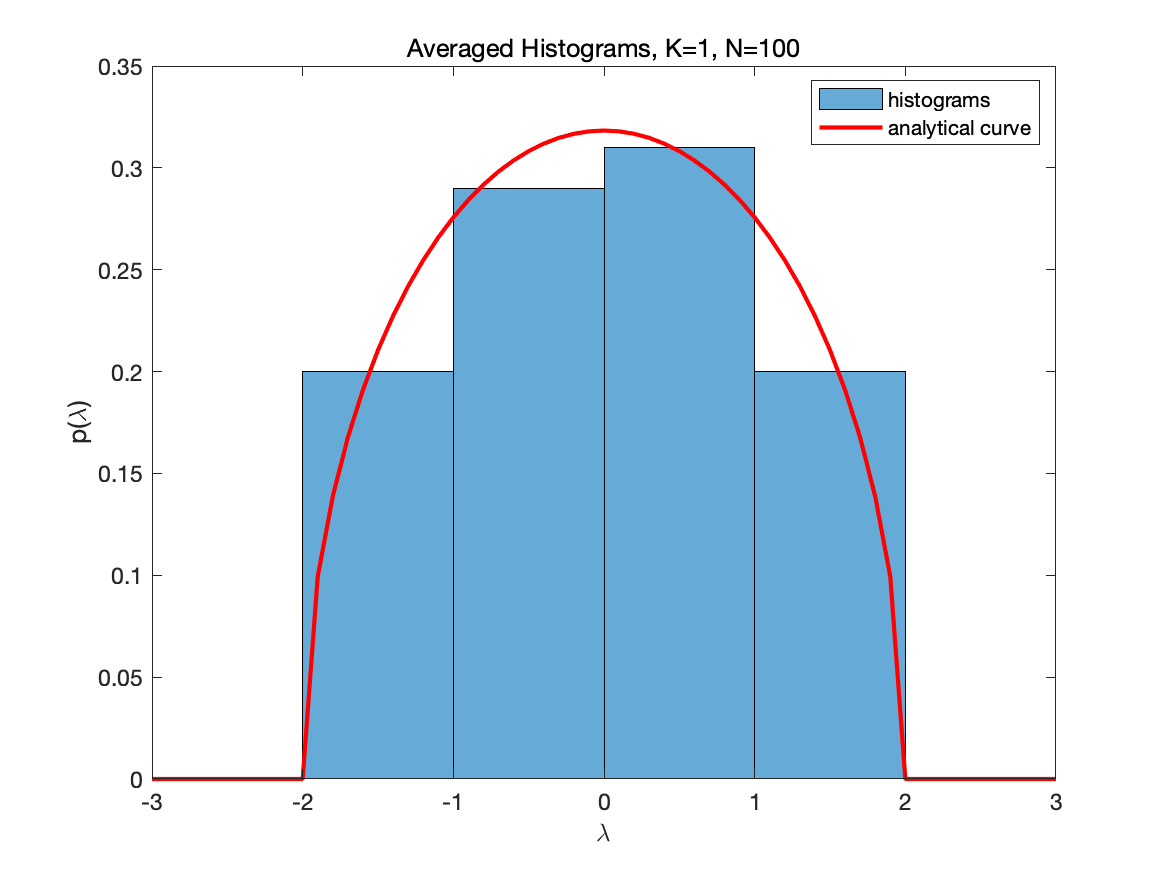
\includegraphics[width=0.49\textwidth]{HW0_1_c_1_100.png}}
\subfigure[K = 1, N = 1000]{\label{subfig:c_b_3}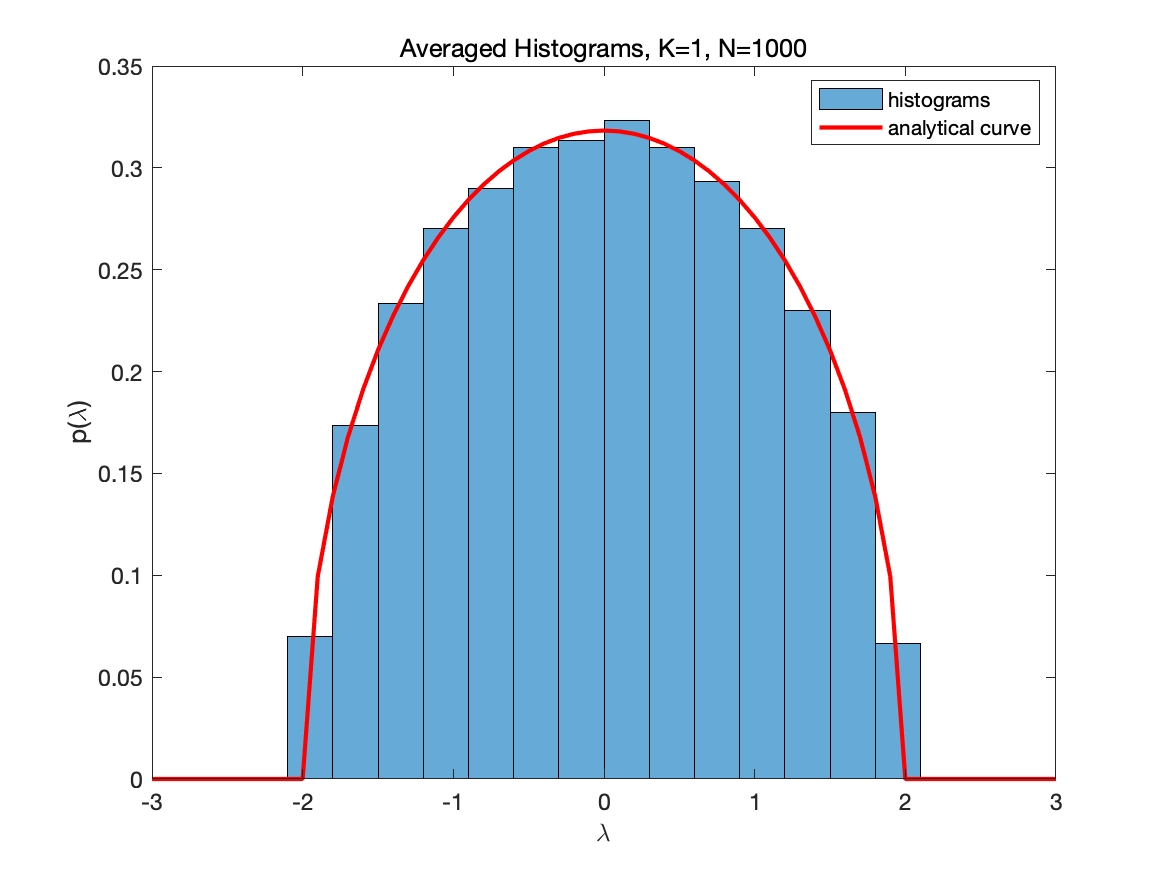
\includegraphics[width=0.49\textwidth]{HW0_1_c_1_1000.png}}
\subfigure[K = 1, N = 4000]{\label{subfig:c_b_4}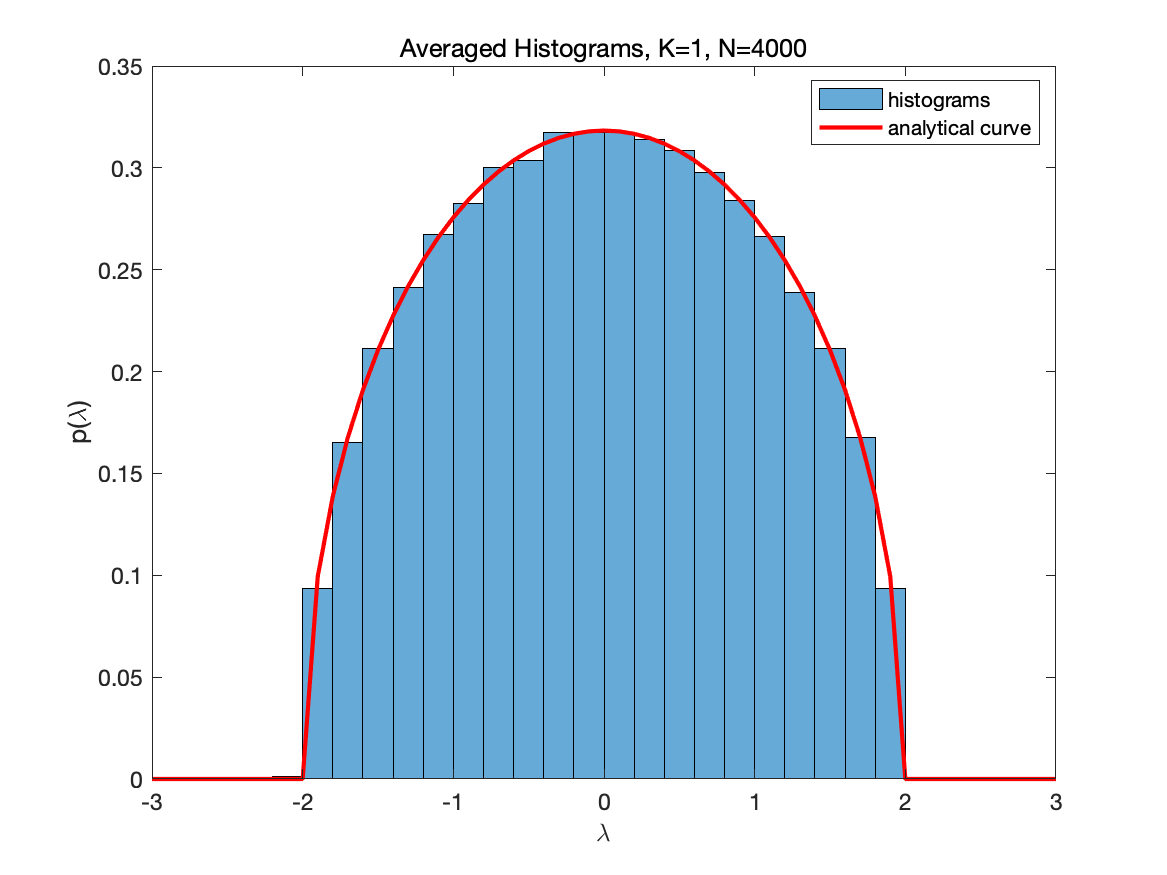
\includegraphics[width=0.49\textwidth]{HW0_1_c_1_4000.png}}
\caption{Averaged histograms and analytical curve, convergence (b)}
\label{fig:c_b}
\end{figure*}

\newpage
\subsection*{(d)}
\textbf{Ans:}\\
The convergence in P2(a) is through increasing the number of different matrices, while the convergence in P2(b) is through increasing the dimension of one matrix. \\
From Figure \ref{fig:c_a} and Figure \ref{fig:c_b}, it is obvious that the frequency histograms will converge to analytical curve with the increase of number of eigenvalues. This convergence is like Bootstrap Distribution, using the histogram of many samples to estimate a real distribution. \\
In Figure \ref{subfig:c_a_1} and Figure \ref{subfig:c_a_2}, because the number of matrices is very large and the dimension is small, there exists many eigenvalues belonging to interval $[-3,-2]$ and $[2,3]$. But the analytical curve is 0 in those intervals. The convergence is not exactly fitting the analytical curve and has some overshoot outside interval $(-2,2)$\\
In Figure \ref{subfig:c_b_3} and Figure \ref{subfig:c_b_4}, because the dimension of matrix is extremely large, the frequency of eigenvalues falling outside interval $(-2,2)$ is very small. Thus, the convergence will exactly fit the analytical curve. \\
Also, we can find, although with a smaller amount of eigenvalues, the convergence in P1(b) is better than that in P1(a). 
% \newpage


\section*{P2}
\subsection*{(a)}
\textbf{Result:}
\begin{figure}[!h]
\begin{center}
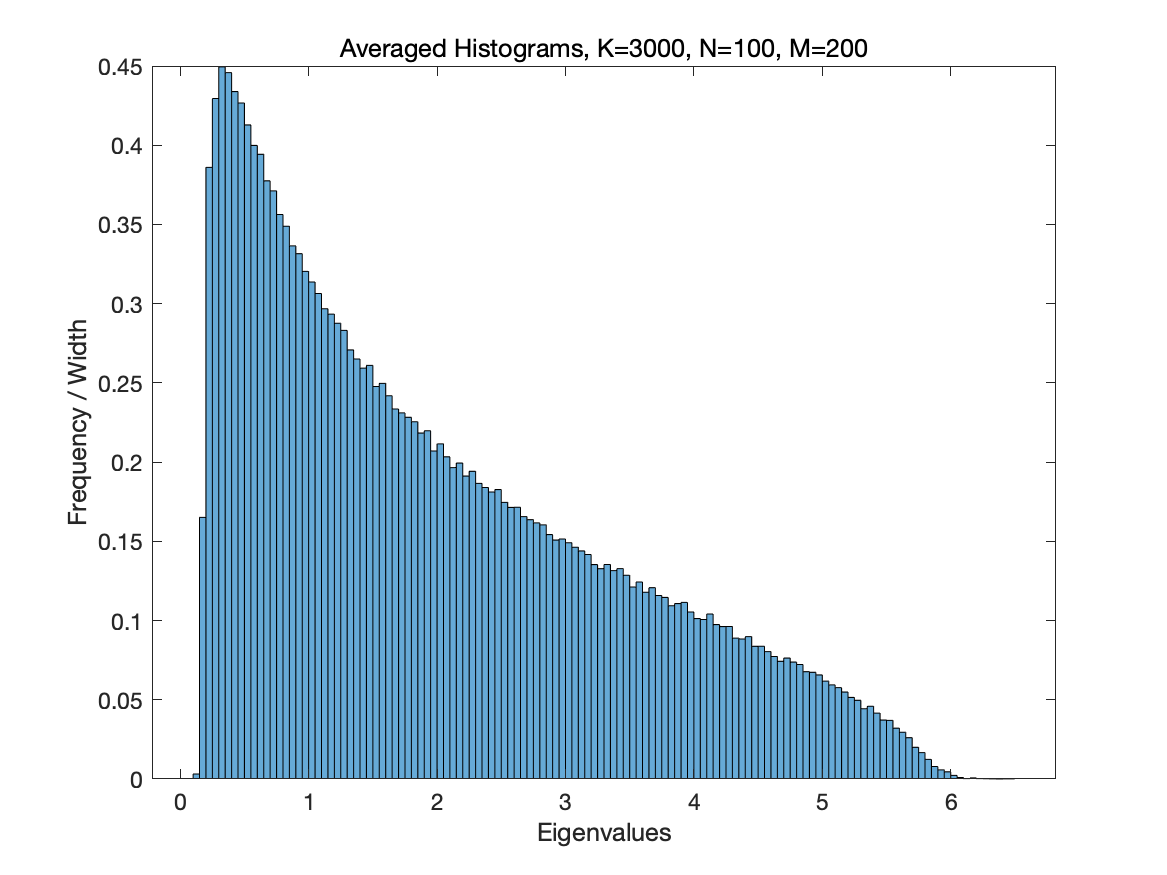
\includegraphics[width=0.95\textwidth]{HW0_2_a_3000_100_200.png}
\end{center}
\caption{Averaged histograms of the eigenvalues of A}
\label{fig:HW0_2_a}
\end{figure}\\
\textbf{Code:}\\
\begin{lstlisting}[language={Matlab}]
K = 3000;
N = 100;
M = 2*N;

% Creat an ensemble of K realizations of N x N Wishart matrices
A = cell(1,K);
for i = 1:1:K
    X = randn(N,M);
    A{i} = (1/N)*(X*X');
end

e = zeros(N,K);
for i = 1:1:K
    e (:, i) = eig(A{i});
end

% Plot a histogram with Normalization set to 'pdf' to produce an estimation of the probability density function.
histogram(e, 'Normalization','pdf')
ylabel('Frequency / Width');
xlabel('Eigenvalues');
title(['Averaged Histograms, K=',num2str(K),', N=',num2str(N),', M=',num2str(M)]);
hold on
saveas(gcf,['/Users/yangchenye/Downloads/HW0_2_a_',num2str(K),'_',num2str(N),'_',num2str(M),'.png'])
\end{lstlisting}


\subsection*{(b)}
\textbf{Code:}
\begin{lstlisting}[language={Matlab}]
K = 1;
N = 2000;
M = 2*N;

% Creat an ensemble of K realizations of N x N Wishart matrices
A = cell(1,K);
for i = 1:1:K
    X = randn(N,M);
    A{i} = (1/N)*(X*X');
end

e = zeros(N,K);
for i = 1:1:K
    e (:, i) = eig(A{i});
end

% Plot a histogram with Normalization set to 'pdf' to produce an estimation of the probability density function.
histogram(e, 'Normalization','pdf')
ylabel('Frequency / Width');
xlabel('Eigenvalues');
title(['Averaged Histograms, K=',num2str(K),', N=',num2str(N),', M=',num2str(M)]);
hold on
saveas(gcf,['/Users/yangchenye/Downloads/HW0_2_b_',num2str(K),'_',num2str(N),'_',num2str(M),'.png'])
\end{lstlisting}
\textbf{Result:}
\begin{figure}[!h]
\begin{center}
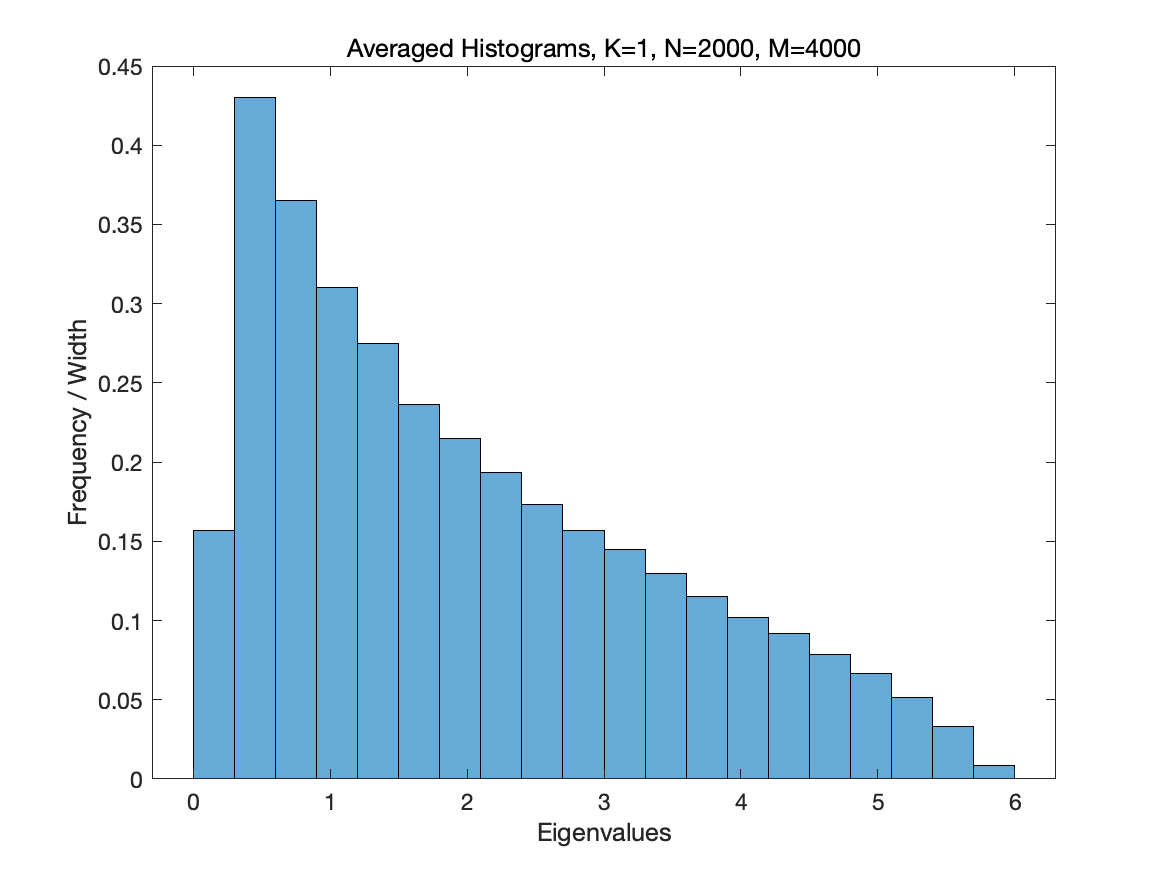
\includegraphics[width=0.95\textwidth]{HW0_2_b_1_2000_4000.png}
\end{center}
\caption{Averaged histograms of the eigenvalues of A}
\label{fig:HW0_2_b}
\end{figure}

\subsection*{(c)}
\textbf{Code:}
\begin{lstlisting}[language={Matlab}]
function [p] = MarcenkoPastur(lamda,N,M)
% Marcenko-Pastur law of the limiting distribution

alpha = M./N;
for i = 1:length(lamda)
    p(i) = sqrt(4*alpha-(lamda(i)-1-alpha).^2)./(2*pi*lamda(i))*(logical((1-sqrt(alpha)).^2 <= lamda(i)) && logical(lamda(i) <= (1+sqrt(alpha)).^2));
end
end
\end{lstlisting}
\begin{lstlisting}[language={Matlab}]
KK = [3000, 1];
NN = [100, 2000];
MM = [2*NN(1), 2*NN(2)];

for question = 1:2
    K = KK(question);
    N = NN(question);
    M = MM(question);
    % Creat an ensemble of K realizations of N x N Wishart matrices
    A = cell(1,K);
    for i = 1:1:K
        X = randn(N,M);
        A{i} = (1/N)*(X*X');
    end

    e = zeros(N,K);
    for i = 1:1:K
        e (:, i) = eig(A{i});
    end

    % Plot a histogram with Normalization set to 'pdf' to produce an estimation of the probability density function.
    histogram(e, 'Normalization','pdf')
    ylabel('p(\lambda)');
    xlabel('\lambda');
    title(['Averaged Histograms, K=',num2str(K),', N=',num2str(N),', M=',num2str(M)]);
    hold on
    plot([0.1:0.1:6], MarcenkoPastur([0.1:0.1:6],N,M), '-r', 'linewidth', 2);
    legend('histograms','analytical curve');
    saveas(gcf,['/Users/yangchenye/Downloads/HW0_2_c_',num2str(K),'_',num2str(N),'_',num2str(M),'.png'])
    close;
end
\end{lstlisting}
\newpage
\textbf{Result:}
\begin{figure}[!h]
\begin{center}
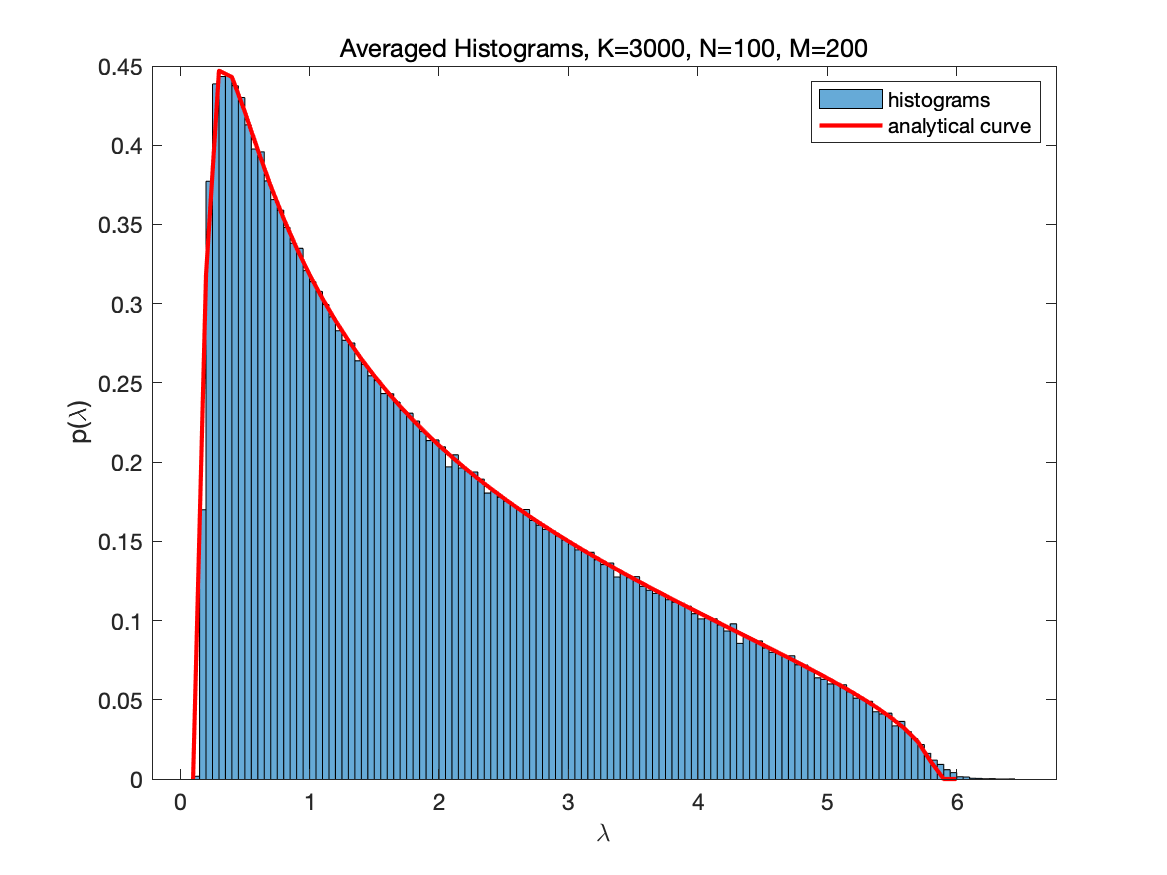
\includegraphics[width=0.70\textwidth]{HW0_2_c_3000_100_200.png}
\end{center}
\caption{Averaged histograms and analytical curve, convergence (a)}
\label{fig:HW0_2_c_a}
\end{figure}
\begin{figure}[!h]
\begin{center}
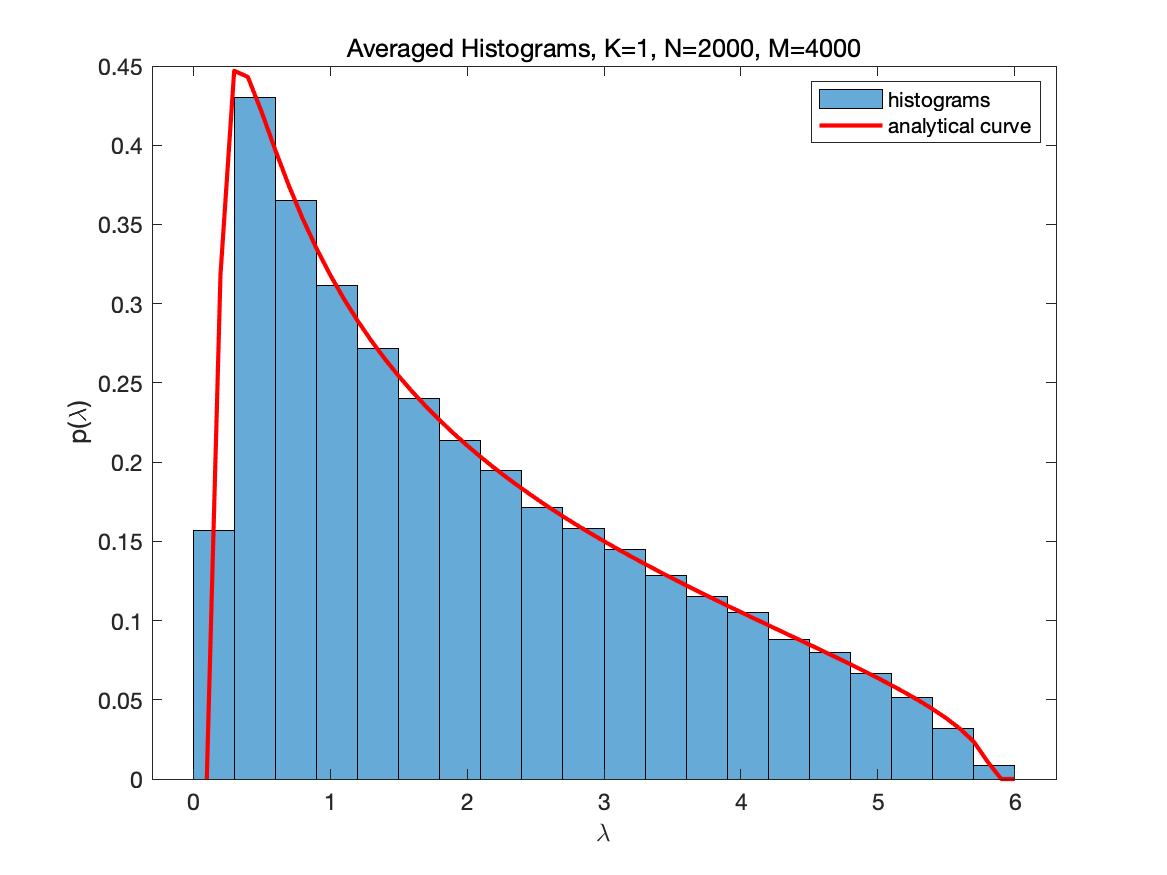
\includegraphics[width=0.70\textwidth]{HW0_2_c_1_2000_4000.png}
\end{center}
\caption{Averaged histograms and analytical curve, convergence (b)}
\label{fig:HW0_2_c_b}
\end{figure}

\subsection*{(d)}
\textbf{Ans:}\\
Firstly, it should be notified that the seemly "difference" between convergence effect is only caused by the bin width of histogram. Plot two histograms with same bin width in one figure bellow (Figure \ref{fig:HW0_2_d}):\\
\begin{figure*}[!h]
\centering
\subfigure[24 bins]{\label{subfig:HW0_2_d_24}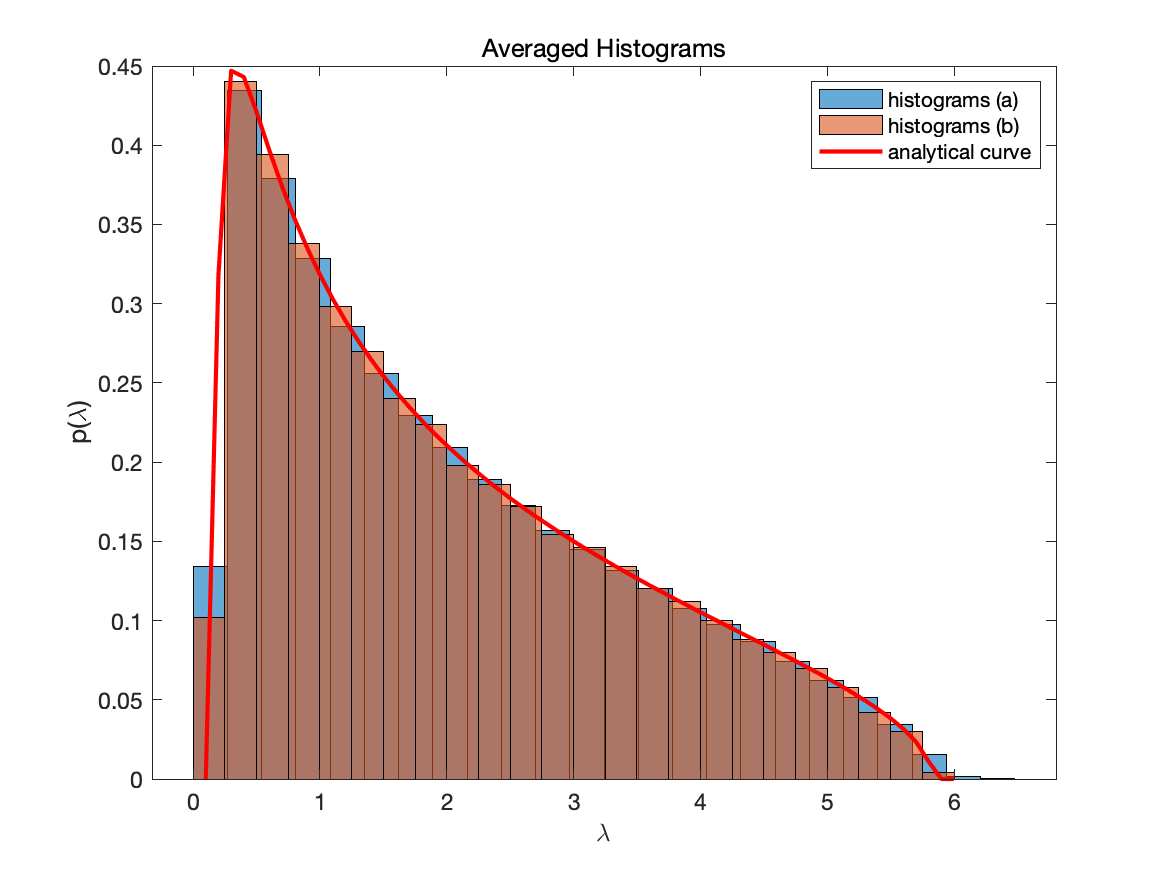
\includegraphics[width=0.49\textwidth]{HW0_2_d_24.png}}
\subfigure[60 bins]{\label{subfig:HW0_2_d_60}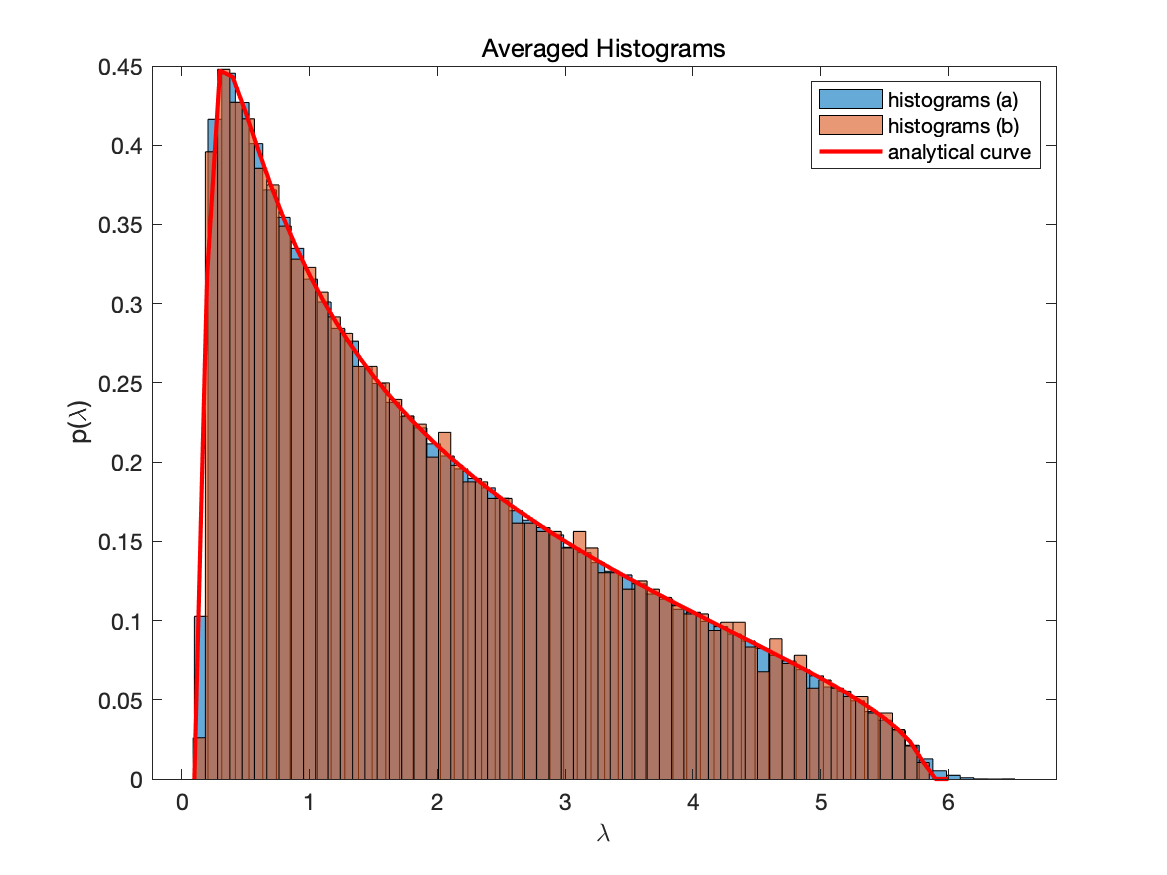
\includegraphics[width=0.49\textwidth]{HW0_2_d_60.png}}
\caption{Different bin width}
\label{fig:HW0_2_d}
\end{figure*}\\
Similarly with Problem 1, the convergence in P2(a) is through increasing the number of different matrices, while the convergence in P2(b) is through increasing the dimension of one matrix. \\
From Figure \ref{fig:HW0_2_c_a} and Figure \ref{fig:HW0_2_c_b}, it is obvious that the frequency histograms will converge to analytical curve with the increase of number of eigenvalues. This convergence is like Bootstrap Distribution, using the histogram of many samples to estimate a real distribution. \\
In Figure \ref{fig:HW0_2_c_a}, because the number of matrices is very large and the dimension is small, there exists many eigenvalues belonging to interval $U(6,\delta)=\{x\ |\ 6-\delta<x<6+\delta\}$. But the analytical curve is 0 in those intervals. The convergence is not exactly fitting the analytical curve and has some overshoot outside interval $(0,6)$\\
In Figure \ref{fig:HW0_2_c_b}, because the dimension of matrix is extremely large, the frequency of eigenvalues falling outside interval $(0,6)$ is very small. Thus, the convergence will exactly fit the analytical curve. \\
Also, from Figure \ref{fig:HW0_2_d}, we can have a clear view that histogram in P2(b) (yellow) has a better convergence than that in P2(a) (blue), even though the total number of eigenvalues in P2(b) is smaller. 






\newpage


\end{document}